\documentclass{book}

\usepackage{textcomp}
\usepackage[T1]{fontenc}
\usepackage{listings}
\usepackage{url}
\usepackage{amsmath}
\usepackage{graphicx}
\usepackage{comment}
\usepackage[tikz]{bclogo}
\usepackage{afterpage}

\usepackage{hyperref}

\usepackage{hyperref}
\hypersetup{
    colorlinks,
    citecolor=black,
    filecolor=black,
    linkcolor=blue,
    urlcolor=black
}

%\usepackage[top=1in, bottom=1in, left=1.3in, right=1.3in]{geometry}

\usepackage{caption}

%\usepackage{trivfloat}

\lstset{ %
columns=fullflexible, % Remove superfluous spaces - copy/pasteable
%%%%%%%%%%%%%%%
%language=bash,                % the language of the code
basicstyle=\footnotesize\ttfamily,       % the size and font that are used for the code
showspaces=false,               % show spaces adding particular underscores
showstringspaces=false,         % underline spaces within strings
showtabs=false,                 % show tabs within strings adding particular underscores
frame=single,                   % adds a frame around the code
tabsize=2,                      % sets default tabsize to 2 spaces
%captionpos=b,                   % sets the caption-position to bottom
breaklines=true,                % sets automatic line breaking
breakatwhitespace=false,        % sets if automatic breaks should only happen at whitespace
%title=\lstname,                 % show the filename of files included with \lstinputlisting;
                                % also try caption instead of title
%escapeinside={\%*}{*)},         % if you want to add a comment within your code
%morekeywords={*,...}            % if you want to add more keywords to the set
upquote=true                    % Use straight quotes
% The following is to make this copy-pasteable (in addition to the upquote and columns, above)
literate={*}{{\char42}}1
         {-}{{\char45}}1
}

% SET UP INVISIBLE (WHITE) CAPTIONS SO I CAN HAVE A TOC FOR BOXES
% NOT ALL THAT ELEGANT, BUT IT WORKS, WHICH IS #1
\usepackage{color}
\DeclareCaptionFont{white}{\color{white}}
\DeclareCaptionType[fileext=lob,placement=b,within=chapter]{boxx}[Box][Boxes]
\DeclareCaptionStyle{mystyle}[margin=0mm,justification=centering]{labelfont={scriptsize,white},font={scriptsize,white},labelfont={scriptsize,white},margin={0mm,0mm}}
%\captionsetup[boxx]{labelfont=white,textfont=white}
%\captionsetup[boxx]{labelfont={white,scriptsize},textfont={white,scriptsize},margin={0mm,0mm}}
\captionsetup[boxx]{style=mystyle}
\begin{comment}
\DeclareCaptionType[fileext=lob,placement=b,within=chapter]{boxx}[Box][List of Boxes]

\renewenvironment{box}
{
  \captionsetup{type=boxx,position=b} %skip BELOW the caption
}
\end{comment}



\title{GRASS GIS for Geomorphologists:\\An Introductory Guide}

\author{Andrew Wickert\\\vspace{12pt}DRAFT Revised for GRASS GIS 7.x.x}

\begin{document}

\maketitle

\tableofcontents
\listofboxxs

\section*{Notes}

\noindent Original draft finished 22 December 2011 \\

\noindent First finished draft completed on 16 April 2012 \\

\noindent These notes are written for GRASS 6.4.X. \\

\section*{License}

\includegraphics[width=5cm]{figures/license/CC-BY-SA_icon.pdf} \\
% vectorized icon from http://upload.wikimedia.org/wikipedia/commons/d/d0/CC-BY-SA_icon.svg
GRASS GIS for Geomorphologists: An Introductory Guide by Andrew D. Wickert is licensed under a \href{http://creativecommons.org/licenses/by-sa/3.0/}{\textcolor{purple}{Creative Commons Attribution-ShareAlike 3.0 Unported License}}. You may freely use it, share it, and change it, so long as the author gets some recognition. And if you want to change it, please let me know! I'd love to have help in maintaining and/or expanding this manual.

\chapter{Introduction}

\section{GIS}

Most of you are probably familiar with GIS, and some of you probably use it very often. But for those of you who don't, GIS stands for "Geographical Information System". It is a software / programming language that is designed to work with data that are displayed spatially---in x,y,z or lat/lon,z coordinates.

Geospatial data take two main forms. {\bf Raster} data are regularly-spaced Cartesian grids. {\bf Vector} data are specified by sets of ungridded x,y,z points that do not necessarily coincide with the position and spacing of raster grids. These can include points, lines, and areas. Raster and vector data types can be used in three dimensions as well, with three dimensional grids and the addition of volume-filling vector elements. The most common geomorphic raster is the digital elevation model (DEM); other common rasters are classified land-use maps and remotely sensed imagery: in general, they represent the intensity of some value across the whole region of interest. Common examples of vector data in geomorphology are river channels (lines), lakes (areas), and sample locations (points).

GIS packages contain a number of tools to work with raster and vector data, make calculations based on them, perform file input/output, reproject data from one coordinate system to another, manage databases of georeferenced information, and create human-readable maps to display the data that the GIS package stores and processes.

Some reasons that geomorphologists use GIS are to:
\begin{enumerate}
	\item Build maps
	\item Display topographic data
	\item Make calculations of topographic features (e.g., hypsometry, curvatures of hillslopes)
	\item Generate features involving water: lakes, rivers, drainage basins, shorelines
	\item Calculate regional values, such as insolation and $^{10}$Be production rates
	\item Calculate and/or show regions of landscape change (e.g., erosion, deposition, glacier retreat) over time
\end{enumerate}

\section{What is GRASS?}

GRASS is the most popular open-source GIS package available. GRASS stands for \emph{Geographic Resources Analysis Support System}. It was first developed in 1982 by the US Army Corps of engineers to be able to perform analyses for the National Environmental Policy Act, with an emphasis on environmental research and monitoring. It was released to the community in the early 90's, and has been a community-driven open source project ever since.

\begin{boxx}[!ht]
\begin{bclogo}[arrondi = 0.1, logo = \bcrosevents]{Why GRASS?}
I use GRASS because it is cross-platform; it is very good at hydrologic analyses; it is very scriptable for easy batch processing, sharing of reproducible analyses, and geospatial integration of numerical models; it is open-source (so I can change components to fit my needs), and because I can share my work with anyone from around the world without being tied down to expensive software. \\
\end{bclogo}
\caption{Why GRASS?}
\end{boxx}

Being open-source means that you can view and change all of the source code---mostly C, with some bash and Python---in which it is written. While I have occasionally tweaked the source code for specialized projects, I almost never have to: in my experience, GRASS is well-vetted and fully-functional.

For more information, go to \url{http://grass.osgeo.org/}.

\subsection{GRASS Interfaces}

GRASS is more of a computational / scripting GIS and less of a point-and-click GIS than ArcGIS. I find this to be an advantage, but for those of you who like point-and-click there are a couple of options. GRASS now has a new interface that is much improved from its old one, which is good for displaying data. For editing vector files, I have found Quantum GIS to be very nice: \url{http://www.qgis.org/}. It can work with GRASS data structures, and therefore be integrated with your GRASS GIS project.

\subsection{Topology}

A major feature of GRASS is that it is a topological GIS. That is, it is impossible to have small gaps or overlaps between vector areas (or ``polygons''). It also forces lines to meet and interact according to some fairly logical rules. This helps for consistency in geologic mapping and allows users to queery vector maps based on their neighbors.

\subsection{File structure}

GRASS creates its own file system. This is more rigid than the way that Arc handles files, but means that you will never lose your GIS files, and you can take your whole folder with you as a bundle. File operations are handled internally by GRASS. There are a large number of import/export options (GDAL, OGR, ASCII, etc.) that can be used to share your work with other GIS applications. I mention the file system again in Section \ref{s:CreateLocation}.

\begin{comment}
\section{Why GRASS?}

There are a lot of reasons to use GRASS. These came from the top of my head. Points 1, 6, and 8 are the three of these below that are the most important to me.

\begin{enumerate}
	\item {\bf Cross-platform:} Mac, Linux, and Windows
	\item {\bf Design for geomorphic and hydrologic analysis:} GRASS was originally designed by the US Army Corps of Engineers, hence its historic strength lies in its abilities for water resources and other natural world analyses. It requires no extra packages to be able to do these.
	\item {\bf Fast hydrologic analysis algorithms:} GRASS implements the Terraflow project from Duke, and its own watershed analysis programs which have now been modified to run even more quickly
	\item {\bf Lots of included tools for analyzing the natural world}: Works with remotely-sensed data, calculates solar radiation, can perform ecological analyses, powerful raster map calculator, 
	\item {\bf Ability to build rasters from LiDAR point clouds}
	\item {\bf File I/O with all GDAL and OGR formats}: This means that basically any data set format, from any GIS package, can be imported or exported to/from GRASS. This includes things like ESRI shapefiles, KML files such as those used by Google Earth, and multiple raster data formats.
	\item {\bf You'll be learning a skill that isn't tied to an extremely expensive software}
	\item {\bf GRASS is heavily used overseas}: While ArcGIS is common in North America, GRASS is used quite a lot in the rest of the world, both because ESRI has a strong influence in the US geospatial industry and because GRASS is free.
	\item {\bf Easy batch processing and script writing}: You can write scripts for batch processing and to be able to reuse old analyses in GRASS with little effort. Indeed, the software is geared towards an easy-to-use command line interface. This was the major draw for me: I need to reconstruct paleohydrologies over the last glacial cycle!
	\item {\bf Active development and open-source}: You can talk to the GRASS user community about problems. And if a tool that you are trying to use doesn't work, you can change it, recompile, and presto! Now it does work.
\end{enumerate}
\end{comment}


\chapter{Downloading and Installing GRASS}

Installation varies from a no-brainer to a difficult task, depending on your operating system. I am going to be giving instructions for how to make the precompiled binaries work. Compiling your own version of GRASS is important if you want to change the source code and/or use the most updated version, but it takes more work. (Pre-compiled binaries are the normal kinds of programs you would install on a computer from a CD or the internet; compiling it yourself means that you download the code and use a compiler, which turns this code into a binary program that your computer can run.) We will be downloading and installing the stable release of GRASS, which right now is GRASS 6.4.1 or GRASS 6.4.2.

For all of these installation instructions, your computer must have access to the internet.

In addition to the version and platforms mentioned, other versions of GRASS can be downloaded from \url{http://grass.osgeo.org/download/software.php}.

\section{Ubuntu (should work for Debian too)}

Open a terminal (CTRL+ALT+t). Type:
%\lstset{language=bash}
\begin{lstlisting}
sudo apt install grass
\end{lstlisting}
Type your password, press "y" for yes, and wait as the computer installs the program and its dependencies.

\section{Mac OS X}

Mac OS versions of GRASS GIS are available here via download or homebrew (a package manager for Mac OS):

\url{https://grass.osgeo.org/download/software/mac-osx/}

\begin{boxx}[!ht]
\begin{bclogo}[arrondi = 0.1, logo = \bcrosevents]{Good things to have for MacOS}
When I run MacOS, I like to use \emph{iTerm} as my terminal application, and a good text editor like \emph{gedit}, \emph{textWrangler}, \emph{Atom}, or \emph{Sublime}.. These all have syntax highlighting and a bunch of nice additions that make programming and scripting easier.
\end{bclogo}
\caption{Good things to have for MacOS}
\end{boxx}

\section{Windows}

Follow the instructions at:

\url{https://grass.osgeo.org/download/software/ms-windows/}

\chapter{Starting GRASS and Creating a Location}

\section{Starting GRASS}

There are two ways to start GRASS GIS. You can click on the provided icon (Mac, Windows, Linux), or (in Linux and---probably---Windows; maybe Mac but I didn't have luck with this back in 2012 when I put the original guide together) you can open a terminal window and type:
\begin{lstlisting}
 grass -wx
\end{lstlisting}
The \url{wx} indicates that you are starting the graphical interface.

If you click on the icon, check if your operating system also opens a terminal window. You may use this or the internal terminal provided within GRASS. I prefer the to use the system default one, but this may not be available on every OS.

Don't worry if you aren't used to using the command prompt: all of the GRASS commands have a very consistent structure and good documentation, and we will discuss those in depth later.

\section{Database manager \label{s:database}}

Your default database manager for vector data is SQLite. SQL is a very common tool for storing and managing databases across industry, science, etc.

\section{Downloading the sample data set}

Download the Gordon Gulch (snow off) digital elevation model:

\url{https://bcczo.colorado.edu/kmz/arc/shapeFiles/czo_1m_gg_snwOff.zip}

Although this is listed as a ``Digital Surface Model'', which could include the elevation of the vegetation canopy, we will treat all grid cells as if they are the elevation of the land surface for these exercises.

\section{Creating a Location: Gordon Gulch \label{s:CreateLocation}}

Once you start GRASS, a graphical window will pop up. If this is your first time using GRASS, it will ask you to define a directory to hold all of your GRASS GIS files. I typically use something like the default (a ``grass'' or ``grassdata'' folder in my home directory).

Once this folder is created, you will see a start-up screen (see Figure \ref{fig:startup_screen}).

\begin{itemize}
	\item Click {\bf Location Wizard}. You should see a window like Figure \ref{fig:location_wizard_start}.
	\item Set the project location to ``GordonGulch'' and the location title to ``Gordon Gulch - Snow Off'' so the location directory on your computer matches that in this documentation.
	\item Click ``next'', and select the ``Read projection and datum terms from a georeferenced data file'' option (Figure \ref{fig:location_wizard_method}). Lots of other projection selection methods are available, but we want to match the projection of the sample data file, and it is easiest to just pull that out of its metadata.
	\item Click ``next'' and then browse to the folder where you have the Gordon Gulch data that you have downloaded. I usually click on the ``hdr'' file (see Figure \ref{fig:location_wizard_import_georeferencing}, but I think that it is smart enough to figure it out no matter which particular file you choose.
	\item Click ``next''. You'll see a summary of your selections. Then click ``Finish''. A window will pop up asking if you want to import the DEM right away. Click ``no'': I'm going to show you how to do this with the command line.
\end{itemize}

\begin{figure}[h]
 \begin{center}
 \includegraphics[width=.9\linewidth]{figures/ubuntu/main_screen.png}
 \caption{GRASS GIS start-up screen on Ubuntu. If you have just installed GRASS, you will have no project locations or mapsets, and your ``Create mapset'', ``Rename mapset'', and ``Start GRASS'' buttons will be grayed out.}
 \label{fig:startup_screen}
 \end{center}
\end{figure}

\begin{figure}[h]
 \begin{center}
 \includegraphics[width=.9\linewidth]{figures/ubuntu/location_wizard_start.png}
 \caption{Location wizard start screen.}
 \label{fig:location_wizard_start}
 \end{center}
\end{figure}

\begin{figure}[h]
 \begin{center}
 \includegraphics[width=.9\linewidth]{figures/ubuntu/location_wizard_method.png}
 \caption{We will be using the metadata with the Gordon Gulch LiDAR file to georeference our map, though you can do this in many ways.}
 \label{fig:location_wizard_method}
 \end{center}
\end{figure}

\begin{figure}[h]
 \begin{center}
 \includegraphics[width=.9\linewidth]{figures/ubuntu/location_wizard_import_georeferencing.png}
 \caption{We will be using the metadata with the Gordon Gulch LiDAR file to georeference our map, though you can do this in many ways.}
 \label{fig:location_wizard_import_georeferencing}
 \end{center}
\end{figure}

Now that you're done, you'll be back at the starting window, but with your new location ``GordonGulch'' defined (Figure \ref{fig:startup_screen_ready}). Inside GordonGulch, there is a mapset called ``PERMANENT''. This is the mapset that you will be using.

\begin{figure}[h]
 \begin{center}
 \includegraphics[width=.9\linewidth]{figures/ubuntu/startup_screen_ready.png}
 \caption{Back at the start window, but all set to go.}
 \label{fig:startup_screen_ready}
 \end{center}
\end{figure}

In collaborative projects the PERMANENT mapset typically contains only communal files, and each of you would have your own mapset created by clicking the ``create mapset'' button. For example, if we were making a geologic map, a DEM, scanned USGS topo sheets, and remotely sensed data products might be in the PERMANENT mapset. I could read these files, but could not write to them or change anyone else's personal mapset. A few of us could then have our own ``contacts'' vector maps that we would work on independently, without risk of changing someone else's work. When we feel that we are done with our respective sections of the map, we could merge our maps into a final ``contacts'' vector layer, and add that to PERMANENT. This basically exists to avoid common file management issues in collaborative work. The reason that we will be each using PERMANENT as our only mapset for this tutorial should now be obvious: you will be the only user of your GIS location.

There is a reason and a big advantage to this initial set-up step. GRASS internally manages its file structure, and keeps all of its data inside subdirectories of this directory. So long as you don't add and delete files from this directory outside of GRASS (unless you really know what you are doing), this keeps everything very well organized: I have never had to mess with any of this. A big advantage of this internal organization is that your GRASS directories are portable: just copy/paste the entire GRASS directory or location folder, and it will be properly set up on another machine without any of those painful broken links to data files.

\section{Starting a GRASS GIS session}

Now that you've finished setting up your location, you're ready to start using GRASS GIS! We will each use the PERMANENT mapset, since we are the sole users of our GIS projects and want access to everything.

Click on ``Start GRASS'' in the start-up window (Figure \ref{fig:startup_screen_ready}). This window will close, and in its place you will have 2 new GRASS windows (Figure \ref{fig:GUI}). These are the display and the layer manager. If you have a command line window open as well, you should see something that looks like Figure \ref{fig:macCLI}

\begin{figure}[h]
 \begin{center}
 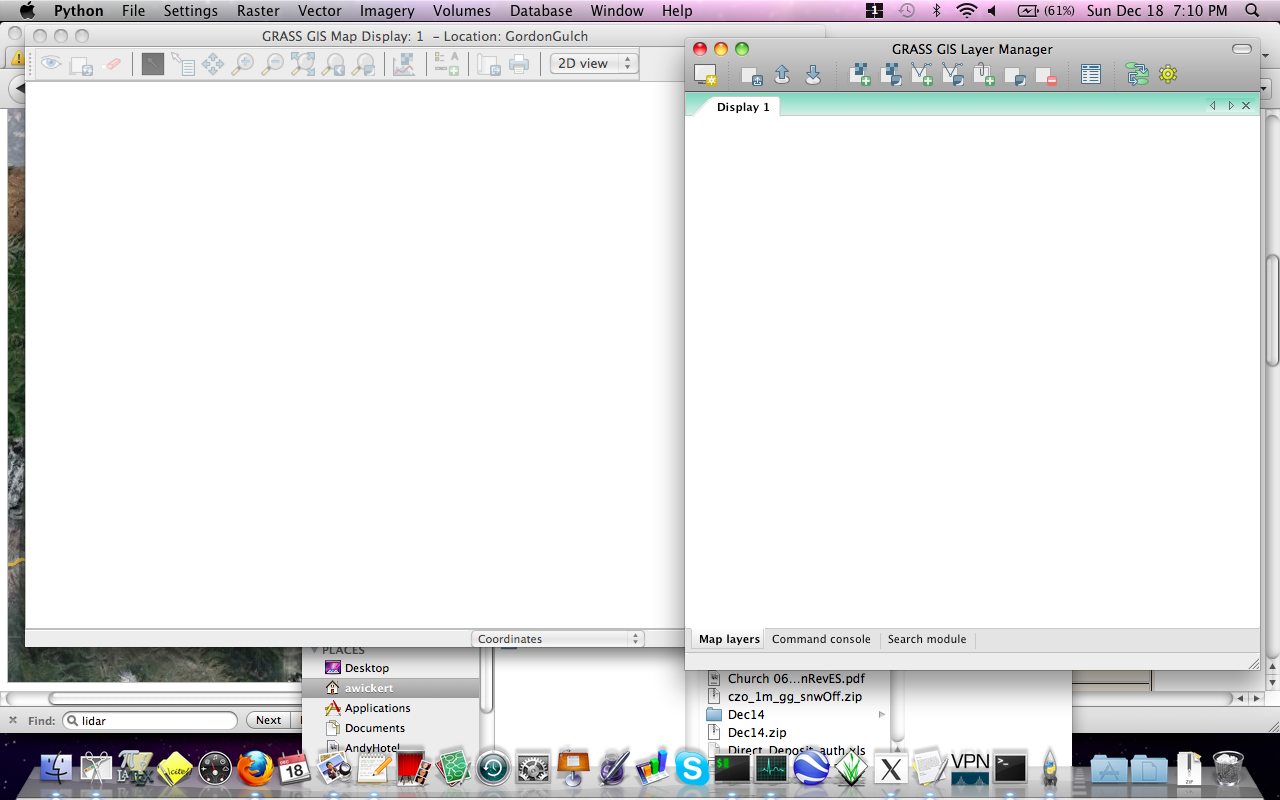
\includegraphics[width=.9\linewidth]{figures/mac/GUI.png}
 \caption{The graphical user interface (GUI) windows in Mac OS. The right-hand window is the layer manager that is the main graphical interface for GRASS. The left-hand window is the map display.}
 \label{fig:GUI}
 \end{center}
\end{figure}

\begin{figure}[h]
 \begin{center}
 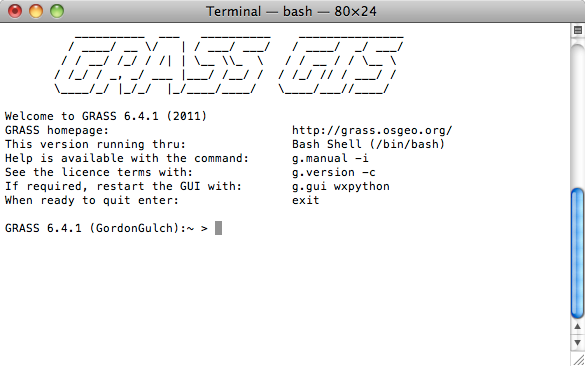
\includegraphics[width=.9\linewidth]{figures/mac/macCLI.png}
 \caption{The command line interface (CLI) in Mac.}
 \label{fig:macCLI}
 \end{center}
\end{figure}


\chapter{Basic Raster Display and Region Operations}

\section{Importing GDAL Raster Data \label{s:importgdal}}

We'll start by importing the DEM with the command line interface. Begin by navigating to the directory where the DEM files are located. For me, this looks like:
\begin{lstlisting}
GRASS 6.4.1 (GordonGulch):~ > cd Documents/geology_docs/courses/GRASS/data/czo_1m_gg_snwOff/czo_1m_gg
GRASS 6.4.1 (GordonGulch):~/Documents/geology_docs/courses/GRASS/data/czo_1m_gg_snwOff/czo_1m_gg > ls
dblbnd.adf  hdr.adf  metadata.xml  prj.adf  sta.adf  w001001.adf  w001001x.adf
\end{lstlisting}
The \url{cd} command changes directory. The \url{ls} command lists the files in the directory. (On Windows this second command is \url{dir}.) The text after the \url{ls} command is the list of files in my DEM directory: if this looks like what you have, then you are in the right place.

The command that you will be using is \url{r.in.gdal}, which imports raster data from any of the common GDAL formats (a GIS standard). Start by typing:
\begin{lstlisting}
 r.in.gdal help
\end{lstlisting}
This brings up a brief manual for that command that should look something like:
\begin{lstlisting}
Description:
 Import GDAL supported raster file into a binary raster map layer.

Keywords:
 raster, import

Usage:
 r.in.gdal [-oeflk] [input=name] [output=name] [band=value]
   [memory=value] [target=string] [title="phrase"] [location=string]
   [--overwrite] [--verbose] [--quiet]

Flags:
  -o   Override projection (use location's projection)
  -e   Extend location extents based on new dataset
  -f   List supported formats and exit
  -l   Force Lat/Lon maps to fit into geographic coordinates (90N,S; 180E,W)
  -k   Keep band numbers instead of using band color names
 --o   Allow output files to overwrite existing files
 --v   Verbose module output
 --q   Quiet module output

Parameters:
     input   Raster file to be imported
    output   Name for output raster map
      band   Band to select (default is all bands)
    memory   Cache size (MiB)
    target   Name of location to read projection from for GCPs transformation
     title   Title for resultant raster map
  location   Name for new location to create
\end{lstlisting}

\begin{boxx}[!ht]
\begin{bclogo}[arrondi = 0.1, logo = \bcrosevents]{Help!}
Typing ``help'' after any command gives a summary of what it does and how it should be used. I have been using GRASS for a long time, and I still do this fairly frequently to make sure that I am using commands correctly, especially when I am working in an interactive session. GRASS has a lot of features, and it can be hard to remember all of the options for all of them!
\end{bclogo}
\caption{Help!}
\end{boxx}

Our import is not going to need to use most of these commands. What we will need to do is to type:
\begin{lstlisting}
 r.in.gdal input=hdr.adf output=topo
\end{lstlisting}
It is possible to shorten the names of the parameters (e.g., ``input'' to ``in'') so long as there is no other parameter that starts with those letters. Once again, I use the \url{hdr.adf} file, though I think that most of them should work for this import. Actually using this command should look something like this:
\begin{lstlisting}
GRASS 6.4.1 (GordonGulch):~/Documents/geology_docs/courses/GRASS/data/czo_1m_gg_snwOff/czo_1m_gg > r.in.gdal input=hdr.adf output=topo
Projection of input dataset and current location appear to match
 100%
r.in.gdal complete. Raster map <topo> created.
GRASS 6.4.1 (GordonGulch):~/Documents/geology_docs/courses/GRASS/data/czo_1m_gg_snwOff/czo_1m_gg > 
\end{lstlisting}

This command starts with ``r'' because it operates on rasters. GRASS uses these ``X.'' beginnings of commands to help differentiate the types of data on which they operate.

\begin{boxx}[!ht]
\begin{bclogo}[arrondi = 0.1, logo = \bcrosevents]{UNIX/GRASS terminal syntax}
Spaces separate distinct things in the UNIX terminal, so you can't have spaces around your ``='' signs. In GRASS, these spaces separate inputs to the commands. Variables are evaluated with ``\$'', and strings are concatenated by doing nothing special. For example:
\begin{lstlisting}
tmp = "testing"
d.mon x0 # open display monitor
d.rast $tmp # display "testing" raster, if it exists
d.out.file -t format=png output=$tmp_file # outputs "testing_file.png" --> d.out.file adds the extension
\end{lstlisting}
\end{bclogo}

Options sent to GRASS GIS commands can be shortened, if unambiguous. For example: ``column'' to ``col'', ``input'' to ``in'', ``output'' to ``out'', ... \\

Flags with one hyphen can be combined (e.g., ``-g -n'' = ``-gn''), and I typically put these before the main commands. I typcally put flags with two hyphens after commands; the most commonly-used of these is the overwrite flag, ``--o''. If this flag is not set, files will not be overwritten.
\caption{UNIX/GRASS terminal syntax}
\end{boxx}


\section{Viewing and setting the region}

All of the commands that you run in GRASS are subject to a particular computational window, which is called the ``region''. You can use the \url{g.region} command to look at the extent of this region and modify it.
\begin{lstlisting}
GRASS 6.4.1 (GordonGulch):~ > g.region -p
projection: 1 (UTM)
zone:       13
datum:      nad83
ellipsoid:  grs80
north:      4431084.5
south:      4428353.5
west:       457305.5
east:       461795.5
nsres:      1
ewres:      1
rows:       2731
cols:       4490
cells:      12262190
\end{lstlisting}
This command gives information on the projection type, region boundaries, and resolution. The current (and default) region is the entire area defined by the Gordon Gulch raster that you used to define the coordinate system. If you change the region and want to bring it back to this full extent and original resolution, type:
\begin{lstlisting}
GRASS 6.4.1 (GordonGulch):~ > g.region rast=topo
\end{lstlisting}
This sets the region to the resolution and edges of the raster ``topo''.

Note that this command starts with a ``g''. These are the general utilities, used for copying data sets, moving them, setting projections, and other general-purpose commands.


\section{Displaying Raster Data}

Now that we know that we have set the computational region to the full extent of the DEM, we are ready to display the data.

\subsection{Simple raster display with the command line}

We will start by viewing the raster data with the command line tool. This isn't as nice/interactive as the GUI, but allows us to write short scripts to create and save map images automatically. This can be nice for creating consistent figures for use in presentations, papers, etc.

We will do some more complex work with both the command line and GUI map displays later on, but for now we will just initialize a window and display the raster DEM.
\begin{lstlisting}
d.mon start=x0 # Start X-windowing display monitor #0
r.colors map=topo color=elevation # Use the scalable elevation color scheme for the topo map
d.rast map=topo # Display the topo map
\end{lstlisting}
When you run these commands, you should have a window appear that looks like Figure \ref{fig:DEMfig}.

\begin{figure}[h]
 \begin{center}
 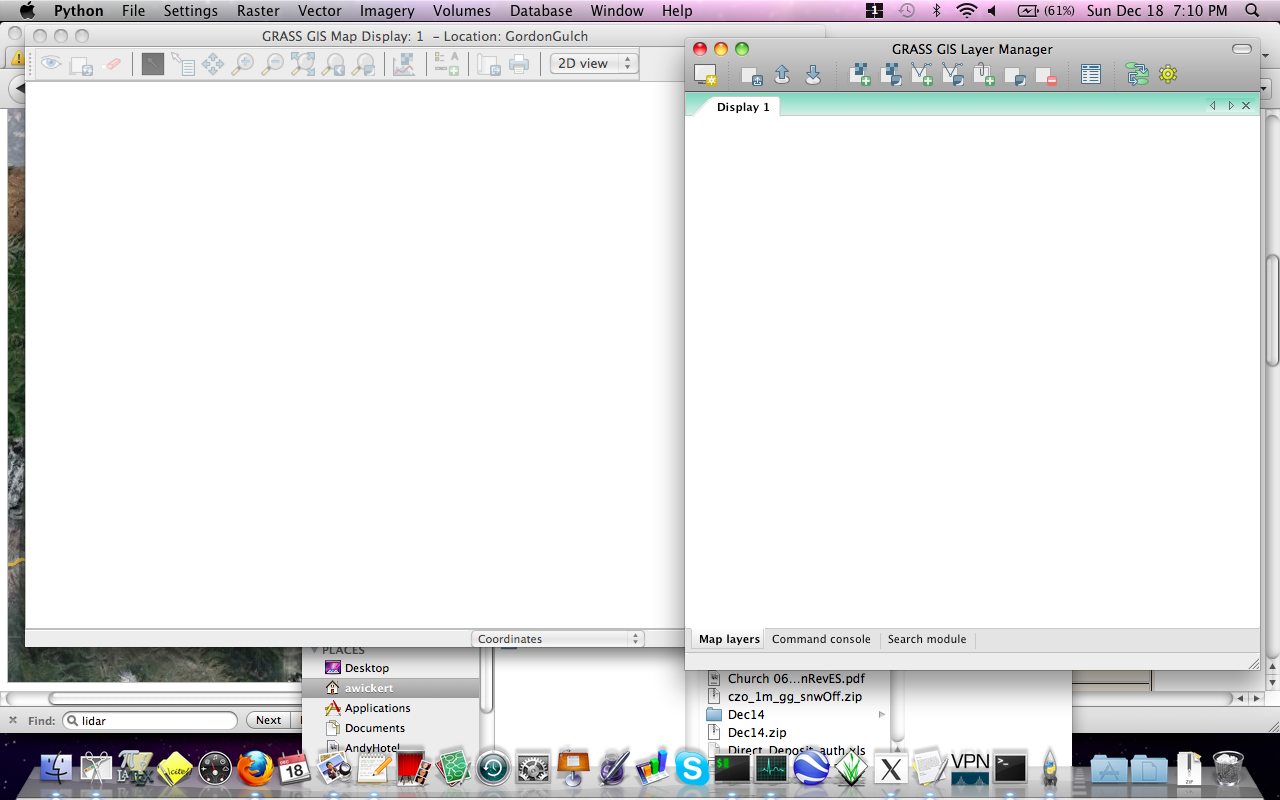
\includegraphics[width=.9\linewidth]{figures/mac/DEMfig.png}
 \caption{A colorized digital elevation model (DEM) of Gordon Gulch in the Boulder Creek Critical Zone Observatory.}
 \label{fig:DEMfig}
 \end{center}
\end{figure}

\subsection{Displaying raster (elevation and shaded relief) maps in the graphical interface}

We can do the same thing in the graphical interface. In the ``GRASS GIS Layer Manager'' window, click on the icon with the checkerboard grid and the plus sign in the top bar. This is the raster display button. A window will appear as soon as you click it (Figure \ref{fig:display_raster}). There should be only one map in the drop down list, our ``topo''. Select it and hit ``OK''. You should now see the LiDAR DEM displayed a second time. If it isn't showing up correctly, you might have to hit the ``zoom to computational region'' button on the GRASS GIS Map Display that goes along with the GUI.

\begin{figure}
 \begin{center}
 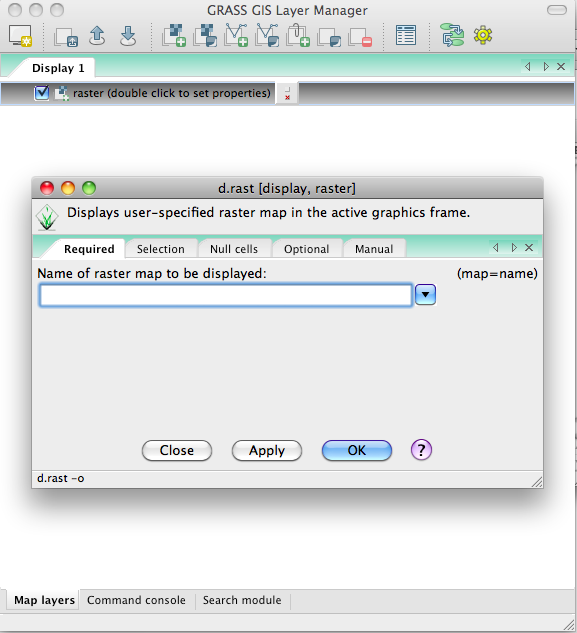
\includegraphics[width=.9\linewidth]{figures/mac/display_raster.png}
 \caption{Displaying raster data in the GUI. Note that the command line command is printed in the lower-left corner. A good way to learn how to script in GRASS is to use the graphical interface and read how what you do graphically relates to what you would type at the command prompt.}
 \label{fig:display_raster}
 \end{center}
\end{figure}

Now, let's add a shaded relief map. Since we have not yet executed any commands other than the map display with the graphical interface, we will use that to construct the shaded relief map. On the menu bar, click {\bf Raster $\rightarrow$ Terrain analysis $\rightarrow$ Shaded relief}. The input elevation map should be ``topo''. Under the ``optional'' tab, set the output shaded relief map name to ``shaded''. Click ``Run''.

This is equivalent to running the following on the command line:
\begin{lstlisting}
 > r.relief map=topo shadedmap=shaded
Calculating shading, please stand by.
 100%
Color table for raster map <shaded> set to 'grey'
Shaded relief map created and named <shaded>.
\end{lstlisting}

We can show the shaded relief map using the GUI. Add the shaded relief map to the layer manager below the ``topo'' DEM. Then right-click on topo and select ``change opacity level''. This cannot be done using the command line in GRASS 6.4 (the command line graphics gets an overhaul in the upcoming GRASS 7.0). I like 30--40\% opacity on the DEM that overlays the shaded relief map.

Now you have a pretty map that combines a DEM with shaded relief to give a good sense of what the topography looks like (Figure \ref{fig:topo_relief_overlay}). If you feel really proud of your map, you can click the ``export image'' button on the toolbar and save it to a file.

\begin{figure}[h]
 \begin{center}
 \includegraphics[width=.9\linewidth]{figures/ubuntu/topo_relief_overlay.png}
 \caption{The gorgeous Gordon Gulch!}
 \label{fig:topo_relief_overlay}
 \end{center}
\end{figure}

\subsection{Combining rasters for display in the command line: elevation and shaded relief \label{s:drastCLI}}

It is also possible to combine raster maps on the command line into a nice-looking result. This allows you to script the generation of maps, which I find especially useful for time-series of data.

I use \url{r.blend} so I can export the resultant set of rasters later on in this tutorial. Another command, \url{d.shadedmap}, works well for draping maps over one another in the display monitor without creating any new rasters. While you can't export the raster directly from the display window, you can also use \url{d.save}, \url{d.out.file}, and other commands to save an image of the current display.

\begin{lstlisting}
# Blend two rasters into a nice result!
r.blend first=topo second=shaded output=colored_shaded_relief percent=40

# This creates a RGB triplet for the shaded relief map that you can display
d.mon x0
d.rgb r=colored_shaded_relief.r g=colored_shaded_relief.g b=colored_shaded_relief.b

# We can use commands to add a title and other nifty features too!
# d.title is used to display the map title and other info; this is 
# in the map's metadata.
# d.text adds selected text
# There are lots of d.* commands to choose from!
\end{lstlisting}

\begin{boxx}[!ht]
\begin{bclogo}[arrondi = 0.1, logo = \bcrosevents]{Tips for the terminal}
If you aren't used to the command prompt, but have a nice terminal emulator, there are some nice tools to know about. The first is autocomplete: press ``tab'' once to complete the current command / file path / etc. you are typing, or at least get it to the point at which it becomes ambiguous as to what you wanted to type. Pressing ``tab'' twice gives you the list of all of the commands / file paths / etc. that start with what you have typed.
\end{bclogo}
\caption{Tips for the terminal}
\end{boxx}


\chapter{Topographic and hydrologic analyses}

\section{Slope, aspect, and resampling \label{s:slope.aspect.resample}}

Let's try another example using the graphical interface (GUI) instead of the command line. We will measure slope and aspect.

Go to the Raster menu. {\bf Raster $\rightarrow$ Terrain analysis $\rightarrow$ Slope and aspect}. Set the raster map to "topo", then click the "outputs" tab. We won't calculate $x$- and $y$- derivatives, as these are in an arbitrary orientation with respect to the hills and valleys. We instead will calculate the slope (steepest decent), aspect, profile (steepest descent orientation) curvature, and tangential (shallowest descent orientation) curvature. I call these "slope", "aspect", "pcurv", and "tcurv", respectively. (See Figure \ref{fig:slope_aspect}.) Look at the bottom. The command-line output is given here. This means that by entering values in the GUI, you can teach yourself how to use the command line -- which is very nice as you start to want to write pre-packaged analysis algorithms. With the GUI window for r.slope.aspect selected, press CTRL+c (or Command+c on mac -- actually, I can't get this to work on mac), and you copy this command-line string:

\begin{lstlisting}
r.slope.aspect elevation=topo slope=slope aspect=aspect pcurv=pcurv tcurv=tcurv
\end{lstlisting}

\begin{figure}[h]
 \begin{center}
 \includegraphics[width=.9\linewidth]{figures/ubuntu/slope_aspect.png}
 \caption{Names for slope and aspect outputs.}
 \label{fig:slope_aspect}
 \end{center}
\end{figure}

Click "run" and it prints out this command line string and runs the desired command.

Try displaying one of the curvature maps in the viewer. It looks like a bunch of random noise (Figure \ref{fig:tcurv1m}). This is because of the high (1 meter) resolution of the LiDAR data: tiny bumps on the surface are dominating the signal. Let's resample these data to 5 meter resolution. First, we have to change our computational region's resolution. Then we use the "r.resample" tool to coarsen our raster map.

\begin{figure}[h]
 \begin{center}
 \includegraphics[width=.9\linewidth]{figures/ubuntu/tcurv1m.png}
 \caption{At 1 meter resolution, local topographic variations completely dominate the curvature signal, removing any obvious signal of the larger-scale landscape.}
 \label{fig:tcurv1m}
 \end{center}
\end{figure}


\begin{lstlisting}
g.region -p nsres=5 ewres=5 # "-p" prints the computational window.
r.resample input=topo output=topo5m
\end{lstlisting}

Now let's run r.slope.aspect again:

\begin{lstlisting}
r.slope.aspect elevation=topo5m slope=slope5m aspect=aspect5m pcurv=pcurv5m tcurv=tcurv5m
\end{lstlisting}

That's better. The profile curvature follows the hillslope contours well, and the tangential curvature traces out river channels (Figure \ref{fig:tcurv5m}). Look at the slope maps as well, and how much more continuous and smooth the 5m slope map is than the 1m slope map.

\begin{figure}[h]
 \begin{center}
 \includegraphics[width=.9\linewidth]{figures/ubuntu/tcurv5m.png}
 \caption{At 5 meter resolution, the tangential curvature is still noisy, but channel networks have become visuallly discernable.}
 \label{fig:tcurv5m}
 \end{center}
\end{figure}


\section{Drainage Networks \label{s:drainage_networks}}

Now let's build some drainage networks. By now you have the general idea behind the syntax, so we'll get right to it. We are going to start by building watersheds with a multi-flow-direction algorithm.

\begin{boxx}[!ht]
\begin{bclogo}[arrondi = 0.1, logo = \bcrosevents]{GRASS GIS online (and offline) help}
To learn about the multi-flow-direction algorithm, or most of the other algorithms in GRASS, you can go to their help page. Look at the main GUI window (the one that shows the layers in display or the command line). On its toolbar, click on the rescue ring; this opens a browser window with the GRASS help. \\

The GRASS help index tells you how to use the commands and what research, theories, and/or publications the commands implement. This help often comes with examples and/or diagrams to better explain the situations. \\

In this particular case, we will navigate to the raster command index and look for \emph{r.watershed}, a watershed basin creation program. [NEW REF]
\end{bclogo}
\caption{GRASS GIS online (and offline) help}
\end{boxx}


[FIGURES]

\begin{lstlisting}
g.region -p nsres=1 ewres=1 # Back to 1-m resolution
# Use "r.watershed help" to find out what the various outputs are
# We are using multi-direction flow; you can use single-direction ("SFD")
# by adding a "-s" flag
# Threshold=62500 means that we need an accumulation area > 250x250 cells
# = 250x250 meters = 0.0625 km2 here
r.watershed elevation=topo accumulation=accum_mfd drainage=draindir_mfd basin=basins_mfd stream=streams_mfd threshold=62500
# Thin the channels raster so we can vectorize it
r.thin input=streams_mfd output=streams_mfd_thinned
# And to vector of stream channels
# Vector and raster datasets may have the same name without overwriting each other.
r.to.vect input=streams_mfd_thinned output=streams_mfd
# Now to vectorize drainage basins
r.to.vect input=basins_mfd output=basins_mfd feature=area
\end{lstlisting}

The ``thinning'' step ensures that there are no clumps of pixels, and that a single vector line therefore can be drawn cleanly through the raster during the \url{r.to.vect} step.

\begin{boxx}[!ht]
\begin{bclogo}[arrondi = 0.1, logo = \bcrosevents]{GRASS add-ons}
GRASS GIS has a number of add-ons. These are applications that have not been fully adopted and integrated into the GRASS suite of tools, but that can still be very useful. One of these, \url{r.stream}, is used for the kinds of watershed problems that we are tackling right now. We will be using the built-in GRASS tools in this tutorial, but to learn more about the GRASS add-ons, go to their wiki page: \url{http://grass.osgeo.org/wiki/GRASS_AddOns}.
\end{bclogo}
\caption{GRASS add-ons}
\end{boxx}


While the multiple flow direction algorithm is good for providing a more accurate representation of flow paths, single flow direction is needed for stream profiling. We are also going to relax the threshold drainage area down to 10,000 cells (10,000 m$^2$ = 100x100 meters). Let's do that now.

\begin{lstlisting}
r.watershed elevation=topo accumulation=accum drainage=draindir basin=basins stream=streams threshold=10000
r.thin input=streams output=streams_thinned
r.to.vect input=streams_thinned output=streams
r.to.vect input=basins output=basins feature=area
\end{lstlisting}

Now we have a set of single vector stream lines in the basin, each of which represents a segment of the full river channel.

Where I have been using the threshold, I have been doing so in terms of cells. But if your cell sizes vary, or you want to input real flow contributions from each cell, you can do that by setting the \url{flow} parameter in \url{r.watershed} to the name of a raster map.

Let's cap our calculatory achievments by displaying the SFD streams on top of the color shaded relief via the command line:

\begin{lstlisting}
d.mon x0
# d.vect -c map=basins_mfd type=boundary # These get confusing, but this is how to display area boundaries
d.rgb r=colored_shaded_relief.r g=colored_shaded_relief.g b=colored_shaded_relief.b
d.vect map=streams color=blue
\end{lstlisting}

\section{Gordon Gulch drainage basin from set pour point \label{s:GGbasin}}

We can use the GRASS \url{r.water.outlet} function to build basins from pour points. In the next exercise, we will do that, along with vectorizing the resultant drainage basin.

A pour point is the selected map location from which to calculate the upstream catchment area. This is given by the \url{easting} and \url{northing} values, which I have typed here to be the outlet of Gordon Gulch, thus making us find the largest basin on the map.

When we vectorize the drainage basin area, note that we have to clean the topology by removing small (1-pixel) areas that are created along with the large drainage basin. This sometimes happens when converting from raster to vector. I use \url{v.clean}, a topology cleaning tool, to remove these small areas. If there are small areas without centroids like these that you would actually want to keep, you can try to add centroids to them with the \url{v.centroids} tool.

\begin{lstlisting}
# Gordon Gulch basin. Output: 1=inside basin; 0=outside basin
r.water.outlet easting=461795 northing=4429173 drainage=draindir basin=GGbasin
# Set non-basin cells to NULL
r.null map=GGbasin setnull=0
# Convert raster to vector: Use the "-s" flag if you want to smooth the vector instead
# of having rectangular pixel-shaped edges
r.to.vect in=GGbasin out=GGbasin feature=area
# What? 4 areas created? But only 1 centroid?
# Need to clean topology after raster conversion. All of the areas without
# centroids are just one pixel, so we will use v.clean:
v.clean in=GGbasin out=tmp tool=rmarea thresh=1 --o
# And now we will copy over our GGbasin vector file and remove "tmp",
# all in one fell swoop, with "rename":
g.rename vect=tmp,GGbasin --o
\end{lstlisting}

Let's look at this in the GRASS graphical user interface. First, click on the ``add vector'' button (Figure \ref{fig:addVector}). Then follow the sequence of events in Figures \ref{fig:dispVector}, \ref{fig:hydroPlot}, and \ref{fig:hydroMap} to display the basin.

\begin{figure}[h]
 \begin{center}
 \includegraphics[width=.9\linewidth]{figures/ubuntu/addVector.png}
 \caption{Click on this button to open a GUI \protect\url{d.vect} dialog to display the vector map and select display preferences.}
 \label{fig:addVector}
 \end{center}
\end{figure}

\begin{figure}[!h]
 \begin{center}
 \includegraphics[width=.45\linewidth]{figures/ubuntu/selectVector.png}
 \includegraphics[width=.45\linewidth]{figures/ubuntu/deselectCentroidArea.png}\\
 \vspace{2mm}
 \includegraphics[width=.45\linewidth]{figures/ubuntu/linewidth2.png}
 \caption{Select the vector to display. Then go through the tabs to show only the boundary and make the line width be 2.}
 \label{fig:dispVector}
 \end{center}
\end{figure}

\begin{figure}[!h]
 \begin{center}
 \includegraphics[width=.7\linewidth]{figures/ubuntu/hydroPlot.png}
 \caption{I've added our shaded relief map with topography draped over it and a blue vector map of the streams (calculated with the SFD algorithm) to my map along with the drainage basin.}
 \label{fig:hydroPlot}
 \end{center}
\end{figure}

\begin{figure}[!htb]
 \begin{center}
 \includegraphics[width=.9\linewidth]{figures/ubuntu/addMapElements.png}
 \includegraphics[width=.9\linewidth]{figures/ubuntu/hydroMapScale.png}
 \caption{In the display window of the GUI, I have added a North arrow and scale bar.}
 \label{fig:hydroMap}
 \end{center}
\end{figure}

This is all for now, but we go back to this drainage basin and these streams in Chapter \ref{s:vector}, in which we learn how to work with vector data and database tables.

\afterpage{\clearpage}

\clearpage

\section{Solar radiation}
Another important topographic analysis is solar radiation. GRASS GIS has a \url{r.sun} module that does just this, with all the bells and whistles (direct, diffuse, and reflected radiation, variable surface albedo, atmospheric conditions, etc.)

You will need to have run r.slope.aspect to get the slope and aspect in decimal degrees as inputs to the solar radiation file (Section \ref{s:slope.aspect.resample}).

The following is an example of r.sun usage. I haven't used it too much, so I don't have too much to say about it, but it looks pretty powerful. The help page (\url{http://grass.fbk.eu/gdp/html_grass64/r.sun.html} for GRASS 6.4.X) gives a pretty thorough description of it, as well as a nice bibliography of the literature (largely solar energy papers) from which the \url{r.sun} developers drew. The GRASS wiki page has more information: \url{http://grass.osgeo.org/wiki/R.sun}. I've thought about linking it in with measured temperature data: \url{r.sun} could help to obtain the upper boundary heat flux, and could be a way towards obtaining a realistic distributed thermal history for a region that has limited point measurements.

\begin{lstlisting}
# lat~40, but we don't need this: GRASS knows where we are 
# This process may take several minutes, especially when you are running it for a whole day!
r.sun -s elevin=topo aspin=aspect slopein=slope day=28 beam_rad=beam_irradiation_day insol_time=insolation_time_day diff_rad=diffuse_irradiation_day refl_rad=reflected_irradiation_day

# Let's sum all of the three radiation types for the whole-day option, using the map calculatior:
r.mapcalc "total_irradiation_day28 = beam_irradiation_day + diffuse_irradiation_day + reflected_irradiation_day"

# Given time - segfaults as with 6.4.1: fixed in newer versions (6.4.2 might be release version now, so we could be safe on this)
# Segfault also caused by including latitude as either value or raster
r.sun -s elevin=topo aspin=aspect slopein=slope lat=40 day=28 time=8.0 beam_rad=beam_irradiance_0800 diff_rad=diffuse_irradiance_0800 refl_rad=reflected_irradiance_0800
\end{lstlisting}

As a quick review of plotting with the addition of a legend, and an early introduction to Bash scripting (Section \ref{s:BashScripting}) and file I/O (Chapter \ref{s:FIO}), I am going to run the following script to display and save images of all of the time steps. I am also using a number of plotting bells and whistles as an example of their usage. The output is given in Figure \ref{fig:rad}

\begin{lstlisting}
d.mon x1 # start display monitor
# start a for loop
for radrast in beam_irradiation_day diffuse_irradiation_day reflected_irradiation_day total_irradiation_day28
do
  # "echo" is Bash's cute way of saying "print this to an output"; by default, stdout = terminal window
  # "$" in Bash indicates that a variable should be evaluated; otherwise, it is treated as itself
  # (e.g., radrast = radrast; $radrast = beam_irradiation_day)
  echo $radrast
  d.rast $radrast
  d.title -ds map=$radrast
  d.grid -gw size="0:01" color=white textcolor=black fontsize=16
  d.legend map=$radrast color=black at=15,85,15,18
  d.barscale bcolor=none at=0,93
  # save the image here
  d.out.file -t output=$radrast format=png --o
  sleep 1 # Take a look at it!
  d.erase
done
\end{lstlisting}

\begin{figure}[h]
 \begin{center}
 \includegraphics[width=.45\linewidth]{figures/d.out.file/beam_irradiation_day.png}
 \includegraphics[width=.45\linewidth]{figures/d.out.file/diffuse_irradiation_day.png}
 \vspace{3mm}
 \includegraphics[width=.45\linewidth]{figures/d.out.file/reflected_irradiation_day.png}
 \includegraphics[width=.45\linewidth]{figures/d.out.file/total_irradiation_day28.png}
 \caption{Solar radiation maps for January 28th. Some of the features in the standard GRASS output, like the grid and legend text, are thin and don't show up well in this multi-color figure. This is a weakness of the GRASS automated displays.}
 \label{fig:rad}
 \end{center}
\end{figure}

\section{Cosmogenic dating}

One of the many things on my long to-do list is to create a GRASS GIS program to obtain cosmogenic production rates. While I havne't even started coding this, I'll say a little here about how I would do this in GRASS.

GRASS has a function called \url{r.horizon}. It gets the elevation of the horizon from around a point on a DEM. This, coupled the elevation of the sample and an atmospheric thickness function, should be able to give a production rate with a global-uniform assumption. The point also has an $(x,y)$ position. From this, any spatial variability in cosmogenic production rates should be calculatable.

\chapter{Vectors and databases \label{s:vector}}

\section{Vector topology}

In GRASS GIS, an ``area'' comprises a ``boundary''---a line that encloses it---and a ``centroid''---a point within the area that shows on which side of the line the area exists. Vector attributes for areas are attached to the centroids of these areas. Boundaries are shared between areas, and have their own set of attributes: they know about the areas on either side of them, their lengths, etc.

This is a ``topological'' paradigm for vector files that prevents the slivers and overlaps in vector files that are common in shapefiles. (I think that Arc/Info had topologically correct features, but ArcDesktop stopped doing that, possibly to make our lives more difficult...) Anyway, Figure \ref{fig:vector_paradigms} shows the differences between shapefiles and the topological vectors that GRASS uses. The figures are from the GRASS Wiki, \url{http://grass.osgeo.org/wiki/Digitizing_Area_Features}; this page has more information on vector topology.

\begin{figure}[h]
 \begin{center}
 \includegraphics[width=.45\linewidth]{figures/GRASSwiki/Shape.png}
 \includegraphics[width=.45\linewidth]{figures/GRASSwiki/Grass_vectors.png}
 \caption{GRASS maintains vector topology, with shared boundaries between areas and individual areas defined by centroids. Figures from GRASS Wiki, \protect\url{http://grass.osgeo.org/wiki/Digitizing_Area_Features}.}
 \label{fig:vector_paradigms}
 \end{center}
\end{figure}

Other aspects of GRASS vector topology are that points cannot overlap, and lines should not cross or overlap. The whole point of this is to make sure that there are not redundancies or ambiguities in the vecto data: careful preparation of vector data sets can be hugely important for data processing and interpretation!

\section{Managing databases and uploading vector attributes}

We will learn how to manage vector databases with the \url{GGbasin} vector created in Section \ref{s:GGbasin}. This vector has only 1 area and no shared boundaries, so it is the simplest possible starting point (aside from, well, a point).

My most-commonly used command is \url{v.db.select}. This command prints the database values to the screen (or a file), and optionally filters them according to a SQL queery. Try it out! When I do, this happens:

\begin{lstlisting}
GRASS 6.4.1 (GordonGulch):~/grasstmp > v.db.select GGbasin
cat|value|label
1|1|
\end{lstlisting}

The category, ``cat'', is a unique ID for each vector feature that starts at 1 and goes upward. ``Value'' is 1 from the conversion from raster. ``Label'' is empty, because there was no label attached to the drainage basin raster.

Let's add the area of the drainage basin. To do this, we need to add a column:

\begin{lstlisting}
v.db.addcol map=GGbasin columns="area double precision"
\end{lstlisting}

Check it out: a new column is here!

\begin{lstlisting}
GRASS 6.4.1 (GordonGulch):~/grasstmp > v.db.select GGbasin
cat|value|label|area
1|1||
\end{lstlisting}

Columns can be ``double precision'', ``int'', ``varchar'', or ``date''. Other types exist as well, depending on the database manager being used, but I have never had to use anything but the first three mentioned here.

To put a real value in this column, we must get the vector attribute (known but hidden) into the database table. This uses the command \url{v.to.db}. Makes sense, huh? Vector to database! I choose ``units=k'' for km$^2$.

\begin{lstlisting}
GRASS 6.4.1 (GordonGulch):~/grasstmp > v.to.db map=GGbasin opt=area columns=area units=k
Reading areas...
 100%
Updating database...
 100%
1 categories read from vector map (layer 1)
1 records selected from table (layer 1)
1 categories read from vector map exist in selection from table
1 records updated/inserted (layer 1)
GRASS 6.4.1 (GordonGulch):~/grasstmp > v.db.select GGbasincat|value|label|area
1|1||4.195303
\end{lstlisting}

There we go! This can be used to find neighbors, line slopes, perimeters, and lots more fun stuff. Something I've thought about is writing a slope-area calculation algorithm for a whole landscape... would be very do-able, but I just haven't done it yet!

\section{Advanced Vector and Database Processing}

I thought about subtitling this section \textbf{Streams (lines), Stream Segment Endpoints (points), and Drainage Basins (areas)}. It could also be subtitled \textbf{Manipulating Lines and Points, Using Databases, and File I/O}. So this may make it sound like a mixed bag, but it will make sense when it is all done. The point of it is that we can do a lot of nifty stuff with lines, what we've just learned about getting attribute values, and some basin piping of output to extract drainage basins and/or get some pretty interesting landscape characteristics.

\subsection{Obtaining and cleaning points in stream networks}

Back in Section \ref{s:drainage_networks}, we created a set of vector lines for streams. Each of the lines in this vector extends between the two nearest next tributary junctions, the start of the river system (determined by the drainage threshold we selected), and/or the edge of the map.

We can extract points from this vector using the \url{v.to.points} function. In this case, I am setting the \url{-n} flag to look just at the nodes (endpoints) of the lines. The \url{-v} command would get all of the vertices of the line, and \url{-i} would interpolate between these vertices.

\begin{lstlisting}
v.to.points -n input=streams output=streams_endpoints
# Multiple points at tributary junctions: let's clean the topology
v.clean in=streams_endpoints out=tmp tool=rmdupl
# The current attribute tables do not represent our cleaned vector, so let's drop them
v.db.droptable -f map=tmp layer=1
v.db.droptable -f map=tmp layer=2
# We also caused categories to merge by removing duplicate points; let's
# regenerate them in a nice, sequential list
v.category in=tmp out=tmp2 opt=del --o
v.category in=tmp2 out=tmp opt=add --o
# And now we'll regenerate a new table with our new categories
v.db.addtable map=tmp # Adds a table with just the default "cat" column
# Now that we're done, we will overwrite the input file
g.copy vect=tmp,streams_endpoints --o
\end{lstlisting}

I will now add the positions of those points with \url{v.to.db}, as well as their elevations via queerying the raster map with \url{v.what.rast}. (Getting their locations probably won't be necessary, but it's good practice; note also that you can use \url{v.to.db} to get the start and end points of lines directly, in a database table that is attached to those lines. Cool, huh?)

\begin{lstlisting}
v.db.addcol map=streams_endpoints columns="x double precision, y double precision, z double precision"
v.to.db map=streams_endpoints col=x,y units=meters option=coor
v.what.rast vect=streams_endpoints rast=topo col=z
# Run a quick v.db.select to check on your handiwork
v.db.select streams_endpoints
\end{lstlisting}

Some vector files (not this one) have z-coordinates attached as well, meaning that we could skip the \url{v.what.rast} step and just use \url{col=x,y,z}.

\subsection{Queerying categories}

Let's say we want to find only the point that we used to define the major basin of Gordon Gulch. This point should have the lowest of all of the values in our vector categories---and indeed should likely have the lowest elevation of all the points on the map.

Doing this requires making database queeries. Remember Section \ref{s:database}, way back up top? This is where that becomes important. We defined our database manager as SQLite, which is a useful subset of SQL (``Structured Queery Language''), pronounced ``sequel''. Honestly, I find SQL to be a total pain, but once you understand its (rigid) structure and that it is better than the normal set of database managers out there, you start to put up with it and use it.

SQL can be used to perform queeries. For example, to find the minimum elevation from the set of stream endpoints and assign it to variable ``zmin'', I type:

\begin{lstlisting}
zmin=`echo "SELECT MIN(z) from streams_endpoints" | db.select -c`
# Without the "-c" flag, we would need this to cut off the column name:
# zmin=${zmin:7:${#zmin}} # 
\end{lstlisting}

Now that we have this value, we can find the column that is associated with this and save its $x$ and $y$ coordinates.

\begin{lstlisting}
# First, print it all
echo "SELECT * from streams_endpoints WHERE z=$zmin" | db.select
# Then save the latitude and longitude
GGx=`echo "SELECT x from streams_endpoints WHERE z=$zmin" | db.select -c`
GGy=`echo "SELECT y from streams_endpoints WHERE z=$zmin" | db.select -c`
\end{lstlisting}

The commands with pattern \url{db.*} are the purely-databse-oriented queeries.

We can't do this ``x = MIN(x)'' queery in a single step because a SQL command that returns a single value like MIN() can't be used to queery whole columns. See - sort of a pain! This is one way in which the GRASS Python interface becomes useful: vector data can be ingested as lists, which are waaaay more flexible and a lot less painful to use. But let's keep in 100\% GRASS + Bash to do the rest for now.

Now we can build our watershed from before using entirely vector outputs, without having to pick (by hand) these values.

\begin{lstlisting}
r.water.outlet easting=$GGx northing=$GGy drainage=draindir basin=GGbasinVARxy
\end{lstlisting}

... but if you go to display this raster, you'll find out that it is NOT our big basin! We are looking at a small enough area that the normal assumption that the biggest basin's outlet will have the lowest elevation won't always hold. Interesting!

\subsection{Extracting vector subsets}

Let's use our big basin vector to extract only those streams that are within it. We use \url{v.select} for this.

\begin{lstlisting}
v.select ainput=streams binput=GGbasin operator=overlap output=GGstreams
\end{lstlisting}

Other useful commands that are like this are \url{v.overlay}, which combines (overlays) two vector maps, and \url{v.extract}, which extracts a subset of a vector map based on database queeries.

The output of this command can be produced in the display window (Figure \ref{fig:GGdrainage}):

\begin{lstlisting}
d.mon x0
d.shadedmap reliefmap=shaded drapemap=topo brighten=15
d.vect map=GGstreams color=blue
d.vect map=GGbasin color=black type=boundary width=2
d.text -b size=8 text="Gordon Gulch Drainage" color=black font=romanc
d.barscale bcolor=none at=0,93
\end{lstlisting}

\begin{figure}[h]
 \begin{center}
 \includegraphics[width=.9\linewidth]{figures/ubuntu/GGdrainage.png}
 \caption{Drainage from Gordon Gulch only.}
 \label{fig:GGdrainage}
 \end{center}
\end{figure}

\begin{figure}[h]
 \begin{center}
 \includegraphics[width=.9\linewidth]{figures/ubuntu/GUIqueery.png}
 \caption{The mouse shows how to queery attributes interactively. The DEM shows where the tributaries to Gordon Gulch are cut off by the road in the DEM. It is not immediately obvious to me whether or not culverts still connect the real tributaries to the real mainstem. The blue polyline sitting by itself is an artifact of drainage analysis with these roads: it is the piece of the now-blocked Gordon Gulch tributary drainage that managed to live on the edge between the Gordon Gulch and its would-be tributary basin boundaries, and therefore is included in our nominally Gordon-Gulch-only subset of streams generated with \protect\url{v.select}.}
 \label{fig:GUIqueery}
 \end{center}
\end{figure}

On viewing this, you might notice two tributaries that should flow into the downstream end of Gordon Gulch but don't: this is because of the road that appears in the LiDAR. Look for it when you zoom in. Note that a segment of the ``stream'' along the road ended up in the Gordon Gulch drainage by mistake! We have to fix that. On the GUI, click the Queery command (Figure \ref{fig:GUIqueery}, select either ``display mode'' (will be displayed in the GRASS terminal tab of your layers, etc. window) or ``edit'' mode (will show up in a pop-up window), select the ``GGstreams'' layer, and click on that segment. On my computer, this returns \url{cat : 788}. We want to get rid of this, so we use \url{v.extract} with the \url{-r} flag to invert our selection:

\begin{lstlisting}
g.copy vect=GGstreams,GGstreams_pre_fix # make a backup first
v.extract -r in=GGstreams_pre_fix out=GGstreams where="cat=788" --o
\end{lstlisting}

Voil\`{a}: it's gone!

Now that you have just the streams inside this area, you should be able to use them to generate slope-area relations, to compare with field data, and to extract long profiles from their starting points. We have seen that GRASS is capable of all of these things on its own, but because of the clunkiness of SQL, it may not be the easest way to do it. Therefore, I prefer to run these types of analyses in Python (Section \ref{s:Python}).

\begin{boxx}[!ht]
\begin{bclogo}[arrondi = 0.1, logo = \bcrosevents]{Specifying pour point locations by intersections}
You often want to know the draiange area above a point given by the intersection of the stream and another linear feature (a road, a terrace surface edge that is being incised, etc.). There is a neat little trick to do this that is described in a few places online. The basic idea is to combine the vector line files and then use the topology tool \url{v.clean} to find intersections between lines, and have its ``\url{error}'' output be points that give the intersection locations. We then use these input positions as variable inputs to \url{r.water.outlet}, with the help of a little scripting and piping (see the GRASS Wiki link below and Section \ref{s:BashScripting}). Nifty! This is described online in the following places:
\begin{itemize}
 \item \url{http://grass.osgeo.org/wiki/Creating_watersheds}
 \item \url{http://www.surfaces.co.il/?p=241}
\end{itemize}
\end{bclogo}
\caption{Specifying pour point locations by intersections}
\end{boxx}

\chapter{File input and output \label{s:FIO}}

File input and output is handled through a number of modules, depending on the types of data and/or output desired.

\section{Raster \label{s:FIOrast}}

At the very beginning of this manual (Section \ref{s:importgdal}), we imported raster data with \url{r.in.gdal}. This allows us to import any of the GDAL compatible raster formats. \url{r.in.ascii} allows import of ASCII grids with GRASS headers. There are a lot of input and output commands based on this same \url{r.in.*} or \url{r.out.*} pattern, and they work for everything from SRTM data and ArcGIS grids to Matlab \url{*.mat} files to POV-RAY raytraceable files to images (and lots in-between).

\begin{lstlisting}
GRASS 6.4.1 (GordonGulch):~ > r.in.
r.in.arc      r.in.bin      r.in.mat      r.in.wms      
r.in.ascii    r.in.gdal     r.in.poly     r.in.xyz      
r.in.aster    r.in.gridatb  r.in.srtm     
GRASS 6.4.1 (GordonGulch):~ > r.out.
r.out.arc      r.out.gdal.sh  r.out.png      r.out.tiff     
r.out.ascii    r.out.gridatb  r.out.pov      r.out.vrml     
r.out.bin      r.out.mat      r.out.ppm      r.out.vtk      
r.out.gdal     r.out.mpeg     r.out.ppm3     r.out.xyz      
\end{lstlisting}

We will practice file input and output with the raster maps from Section \ref{s:drastCLI}. If we want to export these data to a file, we need to ``group'' the .r, .g, and .b components together. For this, we use the ``group'' command, which is in the \url{i.*} image processing command set.

\begin{lstlisting}
i.group group=colored_shaded_relief input=colored_shaded_relief.r,colored_shaded_relief.g,colored_shaded_relief.b
\end{lstlisting}

\begin{boxx}[!ht]
\begin{bclogo}[arrondi = 0.1, logo = \bcrosevents]{Image processing}
A large component of GIS work deals with image processing. Grass has a large set of image processing commands that are listed as \url{i.*}. They look pretty nifty to me, but I've never had need to use them. The same principles of GRASS scripting that we have discussed so far apply to these commands.
\end{bclogo}
\caption{Image processing}
\end{boxx}

Now we can export an image of the raster to a file. I like PNG for images because it can have transparency.

\begin{lstlisting}
r.out.gdal in=colored_shaded_relief out=colored_shaded_relief.PNG format=PNG
\end{lstlisting}
Note the message in which the precision of the output is changed to match what PNG can handle.

Let's also output a real GIS format. You can type:
\begin{lstlisting}
r.out.gdal -l
\end{lstlisting}
to get a list of all available formats.

Let's try an Erdas Imagine Image (.img):
\begin{lstlisting}
r.out.gdal in=colored_shaded_relief out=colored_shaded_relief.img format=HFA
\end{lstlisting}

Finally, let's try to export an ASCII file:
\begin{lstlisting}
r.out.ascii in=colored_shaded_relief out=colored_shaded_relief.txt
\end{lstlisting}
Wait a minute: that didn't work! GRASS just told us:
\begin{lstlisting}
ERROR: Raster map <colored_shaded_relief> not found
\end{lstlisting}
3-channel data can be stored in GDAL formats, but not in a single ASCII file. We don't have any raster that is called \url{colored_shaded_relief}: all we have is the group that comprises the (r,g,b) triplet. All right - let's just export our all-day solar intensity map instead:
\begin{lstlisting}
r.out.ascii in=total_irradiation_day28 out=total_irradiation_day28.txt
\end{lstlisting}
Now that works. Note that \url{r.out.ascii} tends to take longer and make bigger files. ASCII is the easiest and most universal to read, but is usually also the largest and clunkiest filetype.

This ASCII file has a GRASS header, allowing it to be read back in and providing georeferencing information. This header can be left out if you chose the ``\url{-h}'' flag. For the groundwater modelers, a ``\url{-m}'' flag writes a MODFLOW-compatible grid.

We'll skip file input, but at this point, you know how the syntax should work.

\section{Vector}

Vector I/O works in the same way as raster I/O. The vector I/O commands are:
\begin{lstlisting}
GRASS 6.4.1 (GordonGulch):~ > v.in.
v.in.ascii      v.in.garmin     v.in.lines      v.in.sites
v.in.db         v.in.geonames   v.in.mapgen     v.in.sites.all
v.in.dxf        v.in.gns        v.in.ogr        v.in.wfs
v.in.e00        v.in.gpsbabel   v.in.region     
GRASS 6.4.1 (GordonGulch):~ > v.out.
v.out.ascii     v.out.gpsbabel  v.out.pov       v.out.vtk
v.out.dxf       v.out.ogr       v.out.svg       
\end{lstlisting}
\url{v.out.ogr} is very useful, because it covers all of the OGR formats. \url{v.out.ascii} writes all of the vector values to a human-readable ASCII text file. In the place of \url{v.out.ascii}, I often pipe the output to a file with \url{v.db.select}, because this allows me to suppress header printing (if I want to) and choose a subset of the data (matching a SQL queery, here to choose only the very highest points).
\begin{lstlisting}
v.db.select -c map=streams_endpoints fs=" " where="z > 2700" > streams_endpoints_subset.txt 
\end{lstlisting}
I have also changed the field separator from the default ``|'' to a space, which is natively friendly with Numpy. You will read more about piping to files in Section \ref{s:BashScripting}.

The ``gpsbabel'' and ``garmin'' vector I/O options are very useful to me, because they let me insert my GPS points into GIS easily.

You can check out this stuff on your own: at this point, you know the syntax, how to get help, etc...

\section{Google Earth}

Google Earth is a popular and easy-to-use digital globe. You can export lat/lon raster and vector data to it. In this section, we will learn how to reproject data in GRASS and export it in a way that works with Google Earth.

\subsection{Coordinate transformation to lat/lon}

Open a new GRASS GIS session (you can exit this current one, \url{GordonGulch}, if you feel like it), and create a new location called \url{GordonGulchLL}. Instead of specifying a coordinate system based on a file, as we did in Section \ref{s:CreateLocation}, we will set our coordinate system based on an EPSG code. Select EPSG code 4326 for WGS84: this is the unprojected latitude and longitude. Don't worry about setting the region: we can do that by queerying our orignal \url{GordonGulch} GRASS Location and finding its boundaries in the new (lat/lon) coordinate system. Once again, we'll be the only users of our GIS project, so we will work in the ``PERMANENT'' mapset. Start GRASS again!

\begin{boxx}[!ht]
\begin{bclogo}[arrondi = 0.1, logo = \bcrosevents]{Latitude and Longitude in GRASS}
GRASS works much better in Lat/Lon than Arc: it can do flow routing, its ability to weight cells differently allows the flow routing to be a function of a variable cell area, and most of its other functions work as well. I have on occasion broken things by crossing the 180 meridian, but the GRASS developers have a one-liner to fix that, so I just inserted that into the \url{C} source and recompiled the module. The beauty of an open-source, completely modular GIS!
\end{bclogo}
\caption{Latitude and Longitude in GRASS}
\end{boxx}

The tool that we will be using is \url{r.proj}. Let's first find out how our DEM, \url{topo}, maps into lat/lon:
\begin{lstlisting}
GRASS 6.4.1 (GordonGulchLL):~ > r.proj -p location=GordonGulch input=topo
Input Projection Parameters:  +proj=utm +no_defs +zone=13 +a=6378137 +rf=298.257222101 +towgs84=0.000,0.000,0.000
Input Unit Factor: 1
Output Projection Parameters:  +proj=longlat +no_defs +a=6378137 +rf=298.257223563 +towgs84=0.000,0.000,0.000
Output Unit Factor: 1
Input map <topo@PERMANENT> in location <GordonGulch>:
Source cols: 4490
Source rows: 2731
Local north: 40:01:44.806776N
Local south: 40:00:15.454626N
Local west: 105:30:00.726619W
Local east: 105:26:51.936402W
\end{lstlisting}
Now that we have this info, we can use it to define our region:
\begin{lstlisting}
g.region -p n=40:01:44.806776N s=40:00:15.454626N w=105:30:00.726619W e=105:26:51.936402W rows=2731 cols=4490
\end{lstlisting}
Note from the output of this command that your E-W resolution is lower (more degrees per cell) than your N-S resolution. This is because latitude and longitude are not equal, and 1 degree of longitude at 40$^\circ$N is less than a degree of latitude at 40$^\circ$N. You still have a regular 1-meter grid, and (if you didn't know it already) discovered a major reason for map projections!

OK - enough blabbing. Let's import our topography grid, shaded relief map, Gordon Gulch basin outline, and the streams within Gordon Gulch proper. I'm going to do this inside for loops again, in Bash. The loops are totally unnecessary, but are just to keep making you get used to Bash scripting (if you aren't already). Educational research shows that giving sneak peeks of concepts before they are formally introduced increases retention!
\begin{lstlisting}
# The output names default to the input ones

for rast in topo shaded
do
  echo $rast
  r.proj location=GordonGulch input=$rast
done

for vect in GGstreams GGbasin
do
  echo $vect
  v.proj location=GordonGulch input=$vect
done
\end{lstlisting}
For the rasters, I did not specify an interpolation method, so it defaulted to ``nearest neighbor''. If we had used \url{r.shaded.relief} in lat/lon coordinates instead of just importing ``\url{shaded}'', we would have needed to specify the ``\url{units}'' option to say that our vertical scale is meters.

Let's do a quick display to make sure that everything converted over correctly. I'm using the same commands that were used to generate Figure \ref{fig:GGdrainage} (printed here again so you don't have to flip back):
\begin{lstlisting}
d.mon x0
d.shadedmap reliefmap=shaded drapemap=topo brighten=15
d.vect map=GGstreams color=blue
d.vect map=GGbasin color=black type=boundary width=2
d.text -b size=8 text="Gordon Gulch Drainage" color=black font=romanc
d.barscale bcolor=none at=0,93
\end{lstlisting}
Check out Figure \ref{fig:GGdrain_latlon} to see our projected map and how it differs from Figure \ref{fig:GGdrainage}.

\begin{figure}[h]
 \begin{center}
 \includegraphics[width=.9\linewidth]{figures/ubuntu/GGdrain_latlon.png}
 \caption{Gordon Gulch in latitude and longitude. Note that there is some whitespace at the edge of the map due to the coordinate transformation into a geographic coordinate system (from a projected one), and that the location looks smooshed in the vertical direction. Now think about this every time you use Google Maps, which is just lat/lon: N-S distances look shorter there than they really are, and by a not-so-insignificant amount!}
 \label{fig:GGdrain_latlon}
 \end{center}
\end{figure}

Now that everything is imported, we are ready to send it out to Google Earth!

\subsection{Vector}

Vector output to Google Earth is easy because KML is an OGR file format. Just use:
\begin{lstlisting}
# in general: v.out.ogr format=kml ...
# in particular, for our files:
v.out.ogr input=GGstreams dsn=GGstreams.kml type=line format=KML 
v.out.ogr input=GGbasin dsn=GGbasin.kml type=boundary format=KML # just the basin edge
\end{lstlisting}
For vector input and output, you use ``dsn'' (data source name) to refer to the vector files, instead of ``input'' or ``output'' (whichever the file happens to be -- output in this case).

Place the output in the \url{googleearth} folder that came with this manual; this will let you have all of your raster and vector outputs in the same place.

\subsection{Raster}

\subsubsection{Raster Export}

We will output our raster as a PNG file, because this preserves transparency in those nodata regions (instead of making ugly white splotches). First, we will have to follow the procedure outlined in Sections \ref{s:drastCLI} and \ref{s:FIOrast} to blend and group the topography--shaded relief combination into a RGB raster.
\begin{lstlisting}
r.blend first=topo second=shaded output=colored_shaded_relief percent=40
i.group group=colored_shaded_relief input=colored_shaded_relief.r,colored_shaded_relief.g,colored_shaded_relief.b
\end{lstlisting}

Then we use what we learned in Section \ref{s:FIOrast} to output this into a single, nice, PNG file with transparency preserved:
\begin{lstlisting}
r.out.gdal in=colored_shaded_relief out=GordonGulchMap.PNG format=PNG
\end{lstlisting}

I haven't found a way in \url{r.out.gdal} to make transparent areas. But the output of \url{r.out.gdal} is white only where it should be transparent, so I use ImageMagick. If you haven't used ImageMagick before, it is 100\% worth getting: very easy command line / batch processing of images. Anyway, here's what I do:
\begin{lstlisting}
mv GordonGulchMap.PNG GordonGulchMap_OpaqueOrig.PNG
convert -fuzz 3% -transparent white GordonGulchMap_OpaqueOrig.PNG GordonGulchMap.PNG
\end{lstlisting}

We now add one additional step. Because our blended output was a PNG, it has no georeferencing information. To fix this, we can use \url{r.out.png} one one of the color channels to produce a ``world file'': an ASCII file that geolocates our image. This is necessary for a Google Earth import.
\begin{lstlisting}
r.out.png -tw colored_shaded_relief.b
\end{lstlisting}
Then copy the world file such that the filename of the copied version corresponds to the blended raster that you want to import.
\begin{lstlisting}
cp colored_shaded_relief.b.wld GordonGulchMap.wld
\end{lstlisting}
After you do this once, you'll know how world files are formatted, so you can just create them on your own. You can also just go to Wikipedia (\url{http://en.wikipedia.org/wiki/World_file}) and learn all you'd ever want to know about them right off the bat! Of course, once you read that, you'll realize that rotation is possible, so that whole transparency thing should have been a non-issue... but I really don't know anything about generating rasters that aren't in a N-S-W-E orientation, so we're stuck with this for now! The good news can be that if you are working entirely in geographic coordinates, you won't ever have to worry about the transparency issue.

\subsubsection{Google Earth Tiling}

Rasters need to be tiled for Google Earth. I've included a Python script that does this. This script, \url{gdal2tiles.py} is a standard part of the GDAL library. It should be in the \url{googleearth} folder that accompanies this manual. We'll write our output to that folder as well.

To run the Python script, you will need to have Python 2.X and (almost certainly) Numpy on your computer. You might also need PIL, the Python Imaging Library. There are also programs with nice graphical interfaces that act as wrappers to \url{gdal2tiles.py}. I haven't used them as much, but MapTiler seems pretty good (\url{http://www.maptiler.org/}; review / notes at \url{https://alastaira.wordpress.com/2011/07/11/maptiler-gdal2tiles-and-raster-resampling/}). We'll go forward in a scripting sort of way though, since I'm sure you can work your way through a GUI!

If you type
\begin{lstlisting}
python gdal2tiles.py --help
# or ./gdal2tiles.py --help
# if it is executable
\end{lstlisting}
and/or execute the script without any arguments, you get a description of how to run it.

We are going to run it now, and send the output to a subfolder of googleearth. This is what this looks like on my computer; you can see that I have created a ``grasstmp'' folder for the outputs we have created thus far.
\begin{lstlisting}
awickert@Cordilleran:~/Documents/geology_docs/courses/GRASS/googleearth$ ./gdal2tiles.py  -t "Gordon Gulch LiDAR" -k ~/grasstmp/GordonGulchMap.PNG ./GordonGulchLidarMap
Generating Base Tiles:
0...10...20...30...40...50...60...70...80...90...100 - done.
Generating Overview Tiles:
0...10...20...30...40...50...60...70...80...90...100 - done.
\end{lstlisting}

The files are organized into levels of zoomed-out-ed-ness; this makes it easier on the computer as you zoom in and out of the region. The KML file created is named, by default, ``doc.kml''. I want it to be more specific, so I change that:
\begin{lstlisting}
mv GordonGulchLidarMap/doc.kml GordonGulchLidarMap/GordonGulchLiDAR.kml
\end{lstlisting}
The file structure as it looks on my computer can be seen in Figure \ref{fig:GoogleEarthLiDAR_file_structure}.

\begin{figure}[h]
 \begin{center}
 \includegraphics[width=.9\linewidth]{figures/ubuntu/GoogleEarthLiDAR_file_structure.png}
 \caption{The Google Earth files are organized in a hierarchical folder structure, with a vector KML file that is loaded by Google Earth and indexes them.}
 \label{fig:GoogleEarthLiDAR_file_structure}
 \end{center}
\end{figure}

You probably noticed that there are lots of other options for \url{gdal2tiles.py} that can be used to put the images on web servers, etc. I've never used them, but I bet they could be pretty great for outreach work, making data available to other researchers or the public, etc.

\subsection{Import into Google Earth}

Your raster and vector outputs should now all be prepared (2 vector, 1 raster) and sit within your \url{googleearth} folder. Good? OK.

Open Google Earth. Go to File $\rightarrow$ Open, and navigate to your files. Click on them and watch them appear in your map! [Hey - Google Earth even zooms you straight in to Gordon Gulch!]

The vector files will need some love to stop being that uniform spindly red. Right-click on the vector layers in your left-hand panel in Google Earth, go to the second tab [Style, Color], and click ``share style''. This way Google Earth knows that it can apply a consistent color scheme to all of these vector objects. Give the vectors your desired color and width. They sure can look nice!

\begin{figure}[h]
 \begin{center}
 \includegraphics[width=.9\linewidth]{figures/ubuntu/GoogleEarthVector.png} \\
 \vspace{5mm}
 \includegraphics[width=.9\linewidth]{figures/ubuntu/GG_3x_vert_exxag.png}
 \caption{Above: top-down view of vector map. Below: perspective view of raster and vector data with 3$\times$ vertical exaggeration. Don't you feel like you're a scientist from the movies, zooming through a mission-critical landscape?}
 \label{fig:GoogleEarthGordonGulch}
 \end{center}
\end{figure}

\chapter{Writing and Executing Scripts \label{s:scripts}}

\section{Text editors for programming}

You will want a good basic text editor for programming. These will highlight and color the portions of the code according to their purpose, and (especially if you haven't programmed before) will make understanding what you are doing much more intuitive. The text editors I have used (or heard good things about) are:

\begin{itemize}
	\item Windows: notepad++
	\item Mac: TextWrangler and gedit
	\item Linux: gedit (comes pre-installed)
\end{itemize}

\section{Shell scripting (Bash) \label{s:BashScripting}}

Bash is an old language that is very nice for creating quick-and-dirty scripts to automate tasks. This section provides an introduction to Bash, some information on regular expressions, and how information can be piped to and from files to make the scripts run.

\begin{lstlisting}[language=Bash]
for file in *.txt
do
  echo $file
done
\end{lstlisting}

\begin{lstlisting}[language=Bash]
# Create an empty file calld "fnames.txt": this is what the ">" 
# without any content on the left side of the ">" does
> fnames.txt
for file in *.txt
do
  # Append new lines with all of the file names you find
  # ">>" means append to file; ">" means create file
  # Here, you are "piping" the output of "echo" into 
  # the file fnames.txt, instead of having it appear 
  # in the standard output (i.e. the terminal window)
  echo $file >> fnames.txt
done
\end{lstlisting}

Inside a GRASS environment, we can use GRASS commands here. Let's start by exporting a list of the raster files that we have:
\begin{lstlisting}
# Get a full list of GRASS raster files, and pipe it to "rasters.txt"
g.list rast > rasters.txt
\end{lstlisting}

Use the \url{vi} (or your preferred) text editor to look at the file.
\begin{lstlisting}
vi rasters.txt
\end{lstlisting}
As you can see, it isn't formatted in a nice way, with each entry on its own line. (Press ``:q'', then ``ENTER'' to exit when you are done viewing.) This calls for a tool called \url{sed}, which can parse regular expressions. We will do a lot of find and replace commands with \url{sed}.

First, let's remove the first, second and last lines:
\begin{lstlisting}
cp rasters.txt rasters.txt.backup # backup copy is good!
sed -i '1 d' rasters.txt # Replace first line with nothing
sed -i '1 d' rasters.txt # Replace second line with nothing (it is now the 1st line!)
sed -i '$ d' rasters.txt # Replace last line with nothing
\end{lstlisting}

Now, let's replace the spaces (any number of them) with newline characters, and then remove blank lines that would be read as supposed raster names.
\begin{lstlisting}
sed -i 's/ \+/\n/g' rasters.txt # Turns the spaces into newlines, and your data into a single column!
sed -i '/^$/d' rasters.txt # Removes blank lines
\end{lstlisting}
Use \url{vi} or another text editor to admire your handiwork!

Now, let's display all of these in order... wait, maybe that isn't a good idea... if you get bored of the display of all of your raster maps, press CTRL+C to stop the process.
\begin{lstlisting}
d.mon x0 # start a display monitor
# Then get the values of the lines
while read line
do
  echo $line # print raster name to screen
  d.rast $line # display that raster!
  sleep 2 # wait two seconds
  d.erase # Erase the monitor
done < rasters.txt # Pipe in the text file for reading
\end{lstlisting}


\section{Python scripting \label{s:Python}}

This section won't be written for some time, but this is how I write most of my large GRASS programs. It allows much easier handling of variables, especially in lists and arrays, than Bash scripting. It also has some nice plotting utilities which can produce really pretty figures (Matplotlib's basemap, made by a scientist at NOAA here in Boulder).

Information on Python scripting can be found on the GRASS wiki at:
\begin{itemize}
 \item \url{http://grass.osgeo.org/wiki/GRASS_and_Python}
 \item \url{http://grass.osgeo.org/wiki/GRASS_Python_Scripting_Library}
 \item \url{http://grass.osgeo.org/wiki/Converting_Bash_scripts_to_Python}
\end{itemize}
These sources are fairly comprehensive and link to additional sources of information. This is a major  reason why I am in no hurry to write this section: good information exists, and once you know GRASS and Python, all you need to know are the Python modules to import and the syntax to access GRASS functionality. These Wiki articles comprise most (almost all?) of what I know (and some more besides: I hadn't seen some of these articles before writing this paragraph, and some have seen significant overhaul in recent weeks/months), and link to the rest of what I use.

The Wiki documentation is skimpy on vector handling (Python is still fairly new to GRASS), but the Python API is largely built, so I have used information from the GRASS programmer's manual (a useful resource in general) to work through these issues. See \url{http://grass.osgeo.org/programming6/namespacepython_1_1vector.html} for the GRASS 6.5 version. I still haven't found a way to write data to GRASS vectors from Python data structures: I can use Python to run the standard GRASS vector commands, though.

The full GRASS Progammer's Manual (6.5, but similar to 6.4, and easily found via a web search) is \url{http://grass.osgeo.org/programming6/pythonlib.html} (here open to the Python section, but with access to the whole thing visible).

Python scripting has also provided me with a way to run my numerical models in a geospatially-registered environment. This is great, because it means that my model results can be compared instantly with real-world data. To get a taste of both GRASS Python scripting and model integration, check out a copy of my flexural isostasy model from the CSDMS subversion repository:

\begin{lstlisting}
svn co https://csdms.colorado.edu/svn/flexure
\end{lstlisting}
 
Go to \url{flexure/trunk} and look at \url{r.flexure.py}. It's still a little rough as of when I'm writing this manual (16 April 2012), but hey -- it works -- and it can be a sign of greater things to come!

\chapter{Wrap-up}

\section{Thoughts from the Author}

I hope that this manual has been useful to you. Please let me know if there is anything that needs to be fixed, if you'd want to help and/or expand it in any way, or if you have other questions or suggestions. I really hope that this helps you to be more efficient at the computer, be able to do more insightful analyses in a shorter period of time, and avoid paying sky-high fees for Arc and bursting into tears as it crashes and burns and takes your day of work with it.

The open-source community in Earth-surface processes is growing, as exemplified by projects like the Community Surface Dynamics Modeling System (CSDMS). As geomorphologists, sedimentologists, land-use dynamicists, and other Earth-surface scientists, we are increasingly able to model complex natural systems, and our capacity for field data collection continues to grow. Combining our work into a GIS---especially an open-source GIS like GRASS that has its own community with goals that are not so different from those that many Earth-surface scientists have---is a way I see into the future of data--model integration that will allow us to better predict future events and expain the Earth's past.

This manual has been an entirely free-time project to introduce the geomorphic community to an open-source, highly-automatable GIS and some of the neat things you can do with it. As such, I won't always be able to answer all questions in a timely manner, but I really, really promise that I will try.

Happy geospatial adventures to all of you!

\vspace{.7cm}
\hspace{2cm}--Andy, 16 April 2012
\vspace{.7cm}
\pagebreak

\section{Useful Resources}

For more information and/or further exploration of open source GIS, check out the following (some of which I have mentioned in the text):
\begin{itemize}
 \item Markus Neteler and Helena Mitasova, 2008, \emph{Open Source GIS: A GRASS GIS Approach}. Third Edition. \url{http://www.grassbook.org/}
 \item the GRASS GIS Wiki, \url{http://grass.osgeo.org/wiki/GRASS-Wiki}
 \item The Open Source Geospatial Foundation, \url{http://www.osgeo.org/}, where you can download the software, learn about it, and 
 \item the main GRASS GIS website, \url{http://grass.osgeo.org/}
 \item Quantum GIS, a nice open-source point-and-click GIS that can plug in to GRASS as an attractive front-end: \url{http://www.qgis.org/}
\end{itemize}

\section{Future Plans}

This section is mostly for the author, but it is written in the text so readers can have an idea of what to (maybe) expect:

\begin{enumerate}
 \item Compilation instructions, files with cflags, etc.
 \item Geomorphic Python examples and some general Python background
 \item Code from specific projects and/or codes that I have written to do generally-useful tasks (e.g., regional-scale stream profiles, terrace identification)
 \item CSDMS and GRASS -- but I need to work with CSDMS first to see if I can create a generic GRASS wrapper for their interfaces, and I would need to have time to do that... 
 \item Write a LaTeX environment to make boldface monospaced font typeset instead of co-opting the URL 
 \item Add a section on interpolating data going from point clouds to grids, and LiDAR processing
 \item Remote sensing: learn it, or talk to someone who knows it, and then write about it
\end{enumerate}

\pagebreak

\section{Contact Information}

\begin{centering}
\noindent Andy Wickert\\
University of Colorado\\
Department of Geological Sciences and\\
Institute of Arctic and Alpine Research\\
\end{centering}
\vspace{12pt}

\begin{centering}
\textbf{Street / package address}
1560 30th Street\\
Boulder, CO 80303\\
\end{centering}
\vspace{12pt}

\begin{centering}
\textbf{Mailing (non-packages) address}
Campus Box 450\\
Boulder, CO 80309-0450\\
\end{centering}
\vspace{12pt}

\begin{centering}
\noindent E-mail: \url{wickert@colorado.edu}\\
Permanent forwarding email: \url{awickert@alum.mit.edu}\\
(because I'm graduating from CU soon-ish... right, Bob?)\\
\end{centering}

\end{document}
